\documentclass{article}

%----
%  Colin Tan
%  Basic setup for homework
%----
%----------------------------------------------------------------------------------------
%	PACKAGES AND OTHER DOCUMENT CONFIGURATIONS
%----------------------------------------------------------------------------------------

\usepackage{fancyhdr} % Required for custom headers
\usepackage{lastpage} % Required to determine the last page for the footer
\usepackage{extramarks} % Required for headers and footers
\usepackage{graphicx} % Required to insert images

\usepackage{listings} % listing codes

\usepackage[per-mode=symbol]{siunitx} % SI units
\usepackage{amsmath, amssymb} % Math

\usepackage{tikz} % Drawing graphs
\usepackage{pgfplots} % Drawing mathematical plots
\usepgfplotslibrary{fillbetween}
\pgfplotsset{compat=1.10} % pgf compatable version
\usepackage{float} % Flotation control

\usepackage{framed} % Framing answers
\usepackage{enumitem} % Customize enumeration style

\usepackage{multicol} % Required for columizing
\usepackage{caption} % For non-numbered captions
\usepackage{subcaption} % for caption of subfigures

\usepackage[us]{datetime} % Print date in US format

% Margins
\topmargin=-0.45in
\evensidemargin=0in
\oddsidemargin=0in
\textwidth=6.5in
\textheight=9.0in
\headsep=0.25in 

\linespread{1.1} % Line spacing

% Set up the header and footer
\pagestyle{fancy}
\lhead{\hmwkAuthorName} % Top left header
\chead{\hmwkClass\ (\hmwkClassInstructor\ \hmwkClassTime): \hmwkTitle} % Top center header
\rhead{\firstxmark} % Top right header
\lfoot{\lastxmark} % Bottom left footer
\cfoot{} % Bottom center footer
\rfoot{Page\ \thepage\ of\ \pageref{LastPage}} % Bottom right footer
\renewcommand\headrulewidth{0.4pt} % Size of the header rule
\renewcommand\footrulewidth{0.4pt} % Size of the footer rule

\setlength\parindent{0pt} % Removes all indentation from paragraphs

%----------------------------------------------------------------------------------------
%	DOCUMENT STRUCTURE COMMANDS
%----------------------------------------------------------------------------------------

% Header and footer for when a page split occurs within a problem environment
\newcommand{\enterProblemHeader}[1]{
	\nobreak\extramarks{#1}{#1 continued on next page\ldots}\nobreak
	\nobreak\extramarks{#1 (continued)}{#1 continued on next page\ldots}\nobreak
}

% Header and footer for when a page split occurs between problem environments
\newcommand{\exitProblemHeader}[1]{
	\nobreak\extramarks{#1 (continued)}{#1 continued on next page\ldots}\nobreak
	\nobreak\extramarks{#1}{}\nobreak
}

\setcounter{secnumdepth}{0} % Removes default section numbers
\newcounter{homeworkProblemCounter} % Creates a counter to keep track of the number of problems

\newcommand{\homeworkProblemName}{}
\newenvironment{homeworkProblem}[1][Problem \arabic{homeworkProblemCounter}]{ % Makes a new environment called homeworkProblem which takes 1 argument (custom name) but the default is "Problem #"
	\stepcounter{homeworkProblemCounter} % Increase counter for number of problems
	\renewcommand{\homeworkProblemName}{#1} % Assign \homeworkProblemName the name of the problem
	\section{\homeworkProblemName} % Make a section in the document with the custom problem count
	\enterProblemHeader{\homeworkProblemName} % Header and footer within the environment
}{
	\exitProblemHeader{\homeworkProblemName} % Header and footer after the environment
}

\newcommand{\problemAnswer}[1]{ % Defines the problem answer command with the content as the only argument
	\noindent\begin{oframed}
		#1
	\end{oframed}
}

\newcommand{\homeworkSectionName}{}
\newenvironment{homeworkSection}[1]{ % New environment for sections within homework problems, takes 1 argument - the name of the section
	\renewcommand{\homeworkSectionName}{#1} % Assign \homeworkSectionName to the name of the section from the environment argument
	\subsection{\homeworkSectionName} % Make a subsection with the custom name of the subsection
	\enterProblemHeader{\homeworkProblemName\ [\homeworkSectionName]} % Header and footer within the environment
}{
	\enterProblemHeader{\homeworkProblemName} % Header and footer after the environment
}

%----------------------------------------------------------------------------------------
%	TITLE PAGE
%----------------------------------------------------------------------------------------

\title{
\vspace{2in}
\textmd{\textbf{\hmwkClass:\ \hmwkTitle}}\\
\normalsize\vspace{0.1in}\small{Due\ on\ \hmwkDueDate}\\
\vspace{0.1in}\large{\textit{\hmwkClassInstructor\ \hmwkClassTime}}
\vspace{3in}
}

\author{\textbf{\hmwkAuthorName}}
\date{\today} % Insert date here if you want it to appear below your name

\usetikzlibrary{shapes.geometric, calc}
%\everymath{\displaystyle}
%----------------------------------------------------------------------------------------
%	NAME AND CLASS SECTION
%----------------------------------------------------------------------------------------

\newdate{DueDate}{11}{03}{2015} % Due date in {dd}{mm}{yyyy}
\newcommand{\hmwkTitle}{Homework\ 6} % Assignment title
\newcommand{\hmwkDueDate}{\dayofweekname{\getdateday{DueDate}}{\getdatemonth{DueDate}}{\getdateyear{DueDate}} \displaydate{DueDate}} % Due date
\newcommand{\hmwkClass}{PHYS\ 161} % Course/class
\newcommand{\hmwkClassTime}{11:00am} % Class/lecture time
\newcommand{\hmwkClassInstructor}{Professor Landee} % Teacher/lecturer
\newcommand{\hmwkAuthorName}{Zhuoming Tan} % Your name

%----------------------------------------------------------------------------------------

\begin{document}

\maketitle
\newpage
%----------------------------------------------------------------------------------------
%	TABLE OF CONTENTS
%----------------------------------------------------------------------------------------

%\setcounter{tocdepth}{1} % Uncomment this line if you don't want subsections listed in the ToC

%\newpage
%\tableofcontents
%\newpage

%----------------------------------------------------------------------------------------
%	PROBLEM 1
%----------------------------------------------------------------------------------------

% To have just one problem per page, simply put a \clearpage after each problem

\begin{homeworkProblem}
	(6.4) \textit{Vector potential for a wire}

	Consider the example in Section 6.3, concerning the vector potential for a long straight wire. Rewrite Eqs.~(6.33) and (6.34) in terms of Cartesian coordinates, and verify that $\nabla\times\mathbf{A}=\mathbf{B}$.
	% Question

	\textbf{Solution}

	Because $r^2=x^2+y^2$, $\cos\theta=\frac{x}{r}$, and $\sin\theta=\frac{y}{r}$, the equation 6.33 could be rewritten as 
	\[
		\mathbf{B}=-\frac{\mu_0 I}{2\pi r}\sin\theta\hat{\mathbf{x}}+\frac{\mu_0 I}{2\pi r}\cos\theta\hat{\mathbf{y}}=-\frac{\mu_0 Iy}{2\pi(x^2+y^2)}\hat{\mathbf{x}}+\frac{\mu_0 Ix}{2\pi(x^2+y^2)}\hat{\mathbf{y}}
	\]
	the equation 6.34 could be rewritten as
	\[
		\mathbf{A}=-\hat{\mathbf{z}}\frac{\mu_0 I}{2\pi}\ln(x^2+y^2)^{1/2}=-\hat{\mathbf{z}}\frac{\mu_0 I}{4\pi}\ln(x^2+y^2)
	\]
	To verify $\nabla\times\mathbf{A}=\mathbf{B}$, from symmetry,
	\[
		\nabla\times\mathbf{A}=\frac{\partial A_z}{\partial y}\hat{\mathbf{x}}-\frac{\partial A_z}{\partial x}\hat{\mathbf{y}}
	\]
	an because
	\[
		\frac{\partial A_z}{\partial y}=-\frac{\mu_0 Iy}{2\pi(x^2+y^2)};\quad-\frac{\partial A_z}{\partial x}=\frac{\mu_0 Ix}{2\pi(x^2+y^2)}
	\]
	it is verified.
\end{homeworkProblem}

%----------------------------------------------------------------------------------------
%	PROBLEM 2
%----------------------------------------------------------------------------------------

\begin{homeworkProblem}
	(6.10) \textit{Rings with opposite currents}

	Two parallel rings have the same axis and are separated by a small distance $\epsilon$. They have the same radius $a$, and they carry the same current $I$ but in opposite directions. Consider the magnetic field at points on the axis of the rings. The field is zero midway between the rings, because the contributions from the rings cancel. And the field is zero very far away. So it must reach a maximum value at some point in between. Find this point. Work in the approximation where $\epsilon\ll a$.
	% Question

	\textbf{Solution}

	From the equation for field on axis
	\begin{equation}\tag{6.53}
		B_z=\frac{\mu_0Ib^2}{2(b^2+z^2)^{3/2}}
	\end{equation}
	the field for this set up on the z axis would be
	\[
		B_z=\frac{\mu_0Ia^2}{2}\left(\frac{1}{(a^2+(z-\epsilon/2)^2)^{3/2}}-\frac{1}{(a^2+(z+\epsilon/2)^2)^{3/2}}\right)
	\]
	the first order Taylor expansion is
	\[
		B_z\approx\frac{\mu_0Ia^2}{2}\frac{3z\epsilon}{\left(a^2+z^2\right)^{5/2}}
	\]
	Now let constant $k=\frac{\mu_0Ia^2}{2}$,
	\[
		\frac{B_z}{k}=\frac{3z\epsilon}{\left(a^2+z^2\right)^{5/2}}
	\]
	So take derivative,
	\[
		\frac{d}{dz}\frac{B_z}{k}=\frac{3\epsilon\left(a^2-4z^2\right)}{\left(a^2+z^2\right)^{7/2}}
	\]
	and let it equals zero. It yields that $z=a/2$. Put this result into the equation, the maximum value is:
	\[
		\frac{24\epsilon\mu_0I}{25\sqrt{5}a^2}
	\]
\end{homeworkProblem}

%----------------------------------------------------------------------------------------
%	PROBLEM 3
%----------------------------------------------------------------------------------------

\begin{homeworkProblem}
	(6.36) \textit{Field at different radii}
	
	A current of 8000 amperes flows through an aluminum rod \SI{4}{\cm} in diameter. Assuming the current density is uniform through the cross section, find the strength of the magnetic field at \SI{1}{\cm}, at \SI{2}{\cm}, and at \SI{3}{\cm} from the axis of the rod.
	% Question

	\textbf{Solution}

	Current density is uniform so $J=\frac{\SI{8e3}{\ampere}}{\pi(\SI{0.04}{\meter})^2}=\frac{\SI{5e6}{\ampere\per\square\meter}}{\pi}$. And because $B=\frac{\mu_0 I}{2\pi r}=\frac{\mu_0 J\pi r^2}{2\pi r}=\frac{\mu_0 Jr}{2}$:
	\begin{itemize}
		\item When $r=\SI{1}{\cm}$, $B=\frac{\SI{4\pi e-7}{\volt\second\per\ampere\per\meter}\times\frac{\SI{5e6}{\ampere\per\square\meter}}{\pi}\times\SI{1e-2}{\m}}{2}=\SI{1e-2}{\volt\second\per\square\meter}=\SI{1e-2}{\tesla}$.
		\item When $r=\SI{2}{\cm}$, $B=\frac{\SI{4\pi e-7}{\volt\second\per\ampere\per\meter}\times\frac{\SI{5e6}{\ampere\per\square\meter}}{\pi}\times\SI{2e-2}{\m}}{2}=\SI{2e-2}{\tesla}$.
		\item When $r=\SI{3}{\cm}$, $B=\frac{\SI{4\pi e-7}{\volt\second\per\ampere\per\meter}\times\frac{\SI{5e6}{\ampere\per\square\meter}}{\pi}\times\SI{3e-2}{\m}}{2}=\SI{3e-2}{\tesla}$.
	\end{itemize}
\end{homeworkProblem}

%----------------------------------------------------------------------------------------
%	PROBLEM 4
%----------------------------------------------------------------------------------------

\begin{homeworkProblem}
	(6.60) \textit{Zero field outside a solenoid}

	We showed in the solution to Problem 6.19 that the magnetic field is zero outside an infinite solenoid with arbitrary (uniform) cross-sectional shape. We can demonstrate this fact in another way, similar in spirit to Problem 1.17.

	Consider a thin cone emanating from an exterior point $P$, and look at the two patches where it intersects the solenoid. Consider also the thin cone symmetrically located on the other side of P (as shown in Fig.~6.48), along with its two associated patches. Show that the sum of the field contributions due to these four patches is zero at $P$.
	\begin{figure}[H]
		\centering
		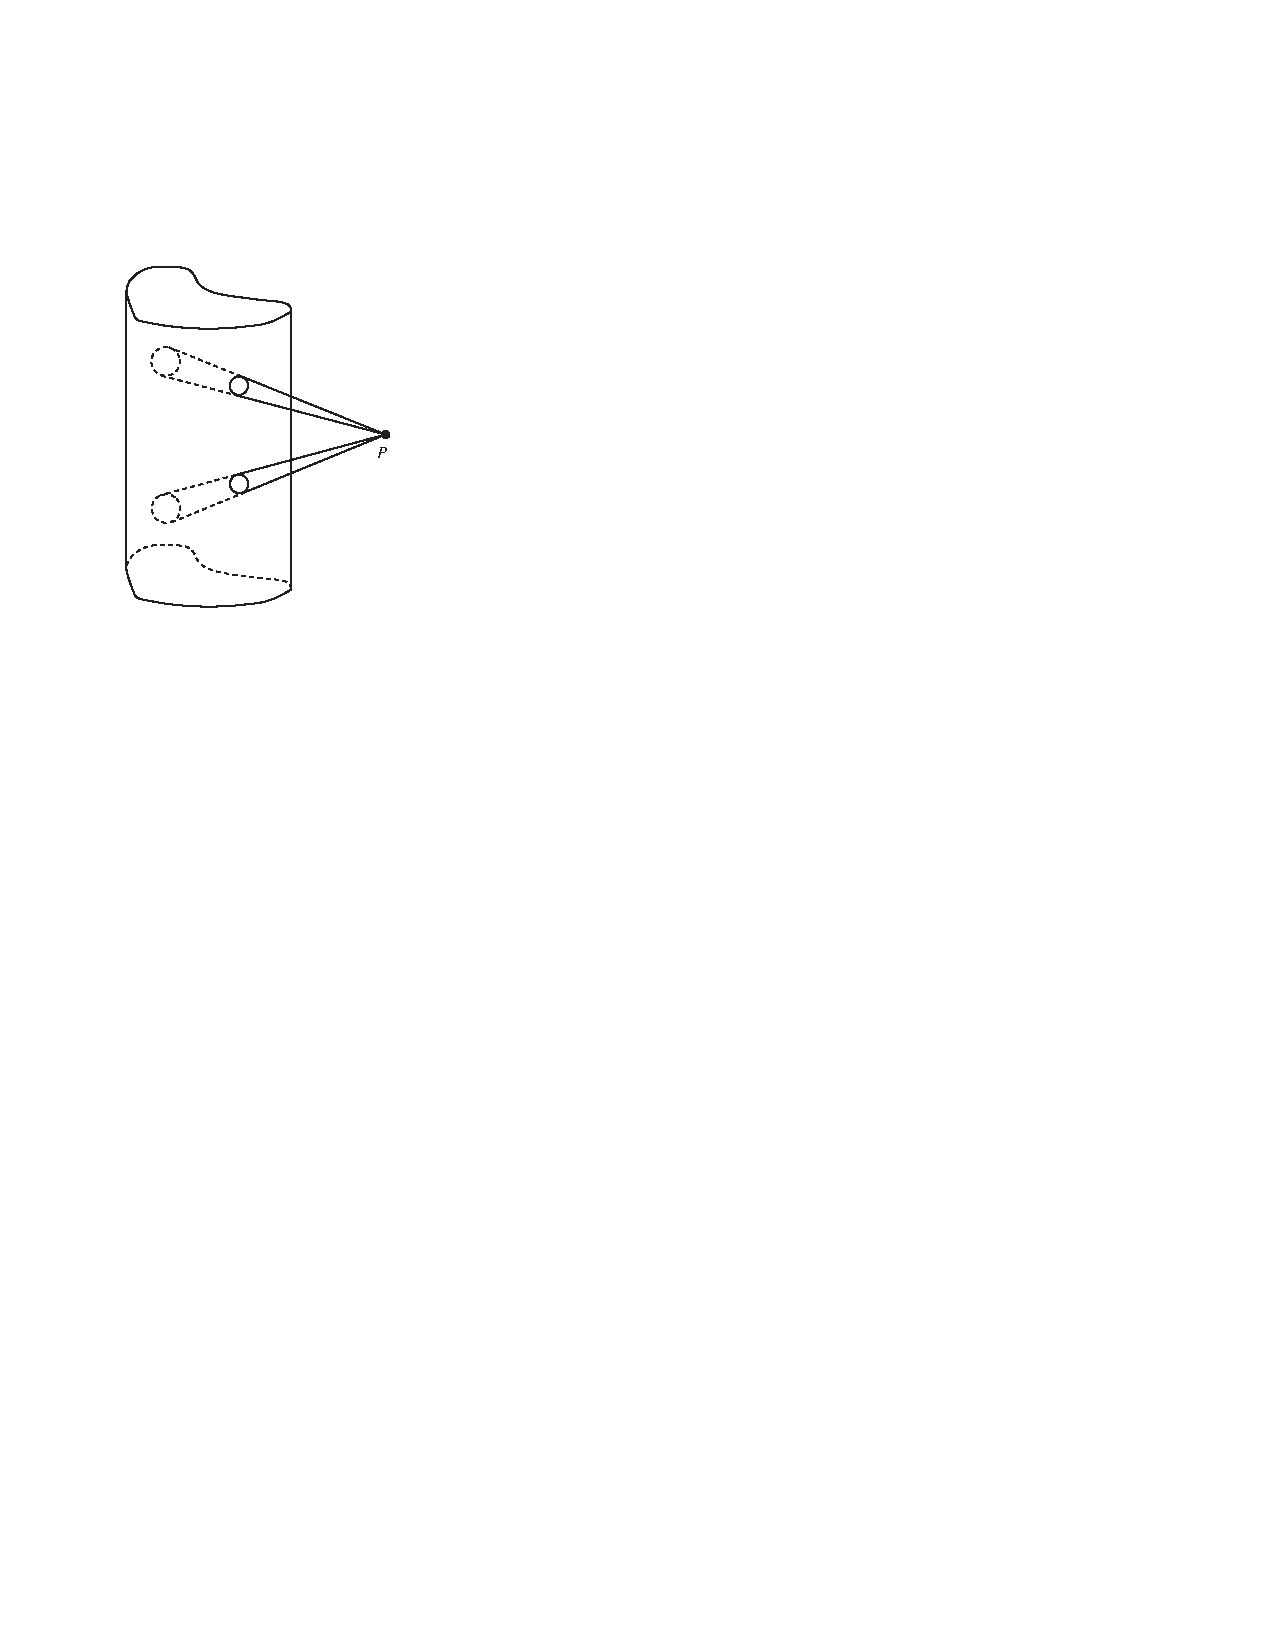
\includegraphics[width = 0.3\textwidth]{6_48.pdf}
		\caption*{Figure~6.48}
	\end{figure}
	% Question

	\textbf{Solution}

	Assume the radius of the solenoid is $R$. The element of the magnetic field
	\[
		d\mathbf{B}=\frac{\mu_0}{4\pi}\frac{I\,d\mathbf{l}\times\hat{\mathbf{r}}}{r^2}
	\]
	By the right hand rule the two patches from the same cone should have contribution to the total field with opposite direction. Let us assume the angle made by the height of the cone and the $z$ axis be $\theta$, and the angle between the height of the cone and the side of the cone $d\phi$, assuming it is small and the obliqueness of the cone is negligible. The current of the closer circle, with the height $r$ is
	\[
		I_1=J(\pi r^2\sin^2d\phi)
	\]
	so
	\[
		dB_1=\frac{\mu_0}{4\pi}\frac{I\,d\mathbf{l}\times\hat{\mathbf{r}}}{r^2}=\frac{\mu_0J}{4\pi}\frac{\pi r^2\sin^2d\phi}{r^2}=\frac{\mu_0J}{4\pi}\sin^2d\phi
	\]
	For the further circle, the height becomes $r+\frac{2R}{\sin\theta}$. So
	\[
		I_2=J\left(\pi\left(r+\frac{2R}{\sin\theta}\right)^2\sin^2d\phi\right)
	\]
	so
	\[
		dB_2=\frac{\mu_0J}{4\pi}\frac{\pi\left(r+\frac{2R}{\sin\theta}\right)^2\sin^2d\phi}{\left(r+\frac{2R}{\sin\theta}\right)^2}=\frac{\mu_0J}{4\pi}\sin^2d\phi
	\]
	They do have the same magnitude and cancel each other out. The same argument applies to the other cone and the two patches of that cone. So the total field should be zero.
\end{homeworkProblem}

%----------------------------------------------------------------------------------------
%	PROBLEM 5
%----------------------------------------------------------------------------------------

\begin{homeworkProblem}
	(6.63) \textit{Solenoids and superposition}

	A number of simple facts about the fields of solenoids can be found by using superposition. The idea is that two solenoids of the same diameter, and length $L$, if joined end to end, make a solenoid of length $2L$. Two semi-infinite solenoids butted together make an infinite solenoid, and so on. (A semi-infinite solenoid is one that has one end here and the other infinitely far away.) Here are some facts you can prove this way.

	\begin{enumerate}[label=(\alph*)]
		\item In the finite-length solenoid shown in Fig.~6.50(a), the magnetic field on the axis at the point $P_2$ at one end is approximately half the field at the point $P_1$ in the center. (Is it slightly more than half, or slightly less than half?)
		\item In the semi-infinite solenoid shown in Fig.~6.50(b), the field line $FGH$, which passes through the very end of the winding, is a straight line from $G$ out to infinity.
		\item The flux of $\mathbf{B}$ through the end face of the semi-infinite solenoid is just half the flux through the coil at a large distance back in the interior.
		\item Any field line that is a distance $r_0$ from the axis far back in the interior of the coil exits from the end of the coil at a radius $r_1=\sqrt{2}r_0$, assuming that $r_0<$(solenoid radius)$/\sqrt{2}$.
	\end{enumerate}
	\begin{figure}[H]
		\centering
		\begin{subfigure}[b]{0.5\textwidth}
			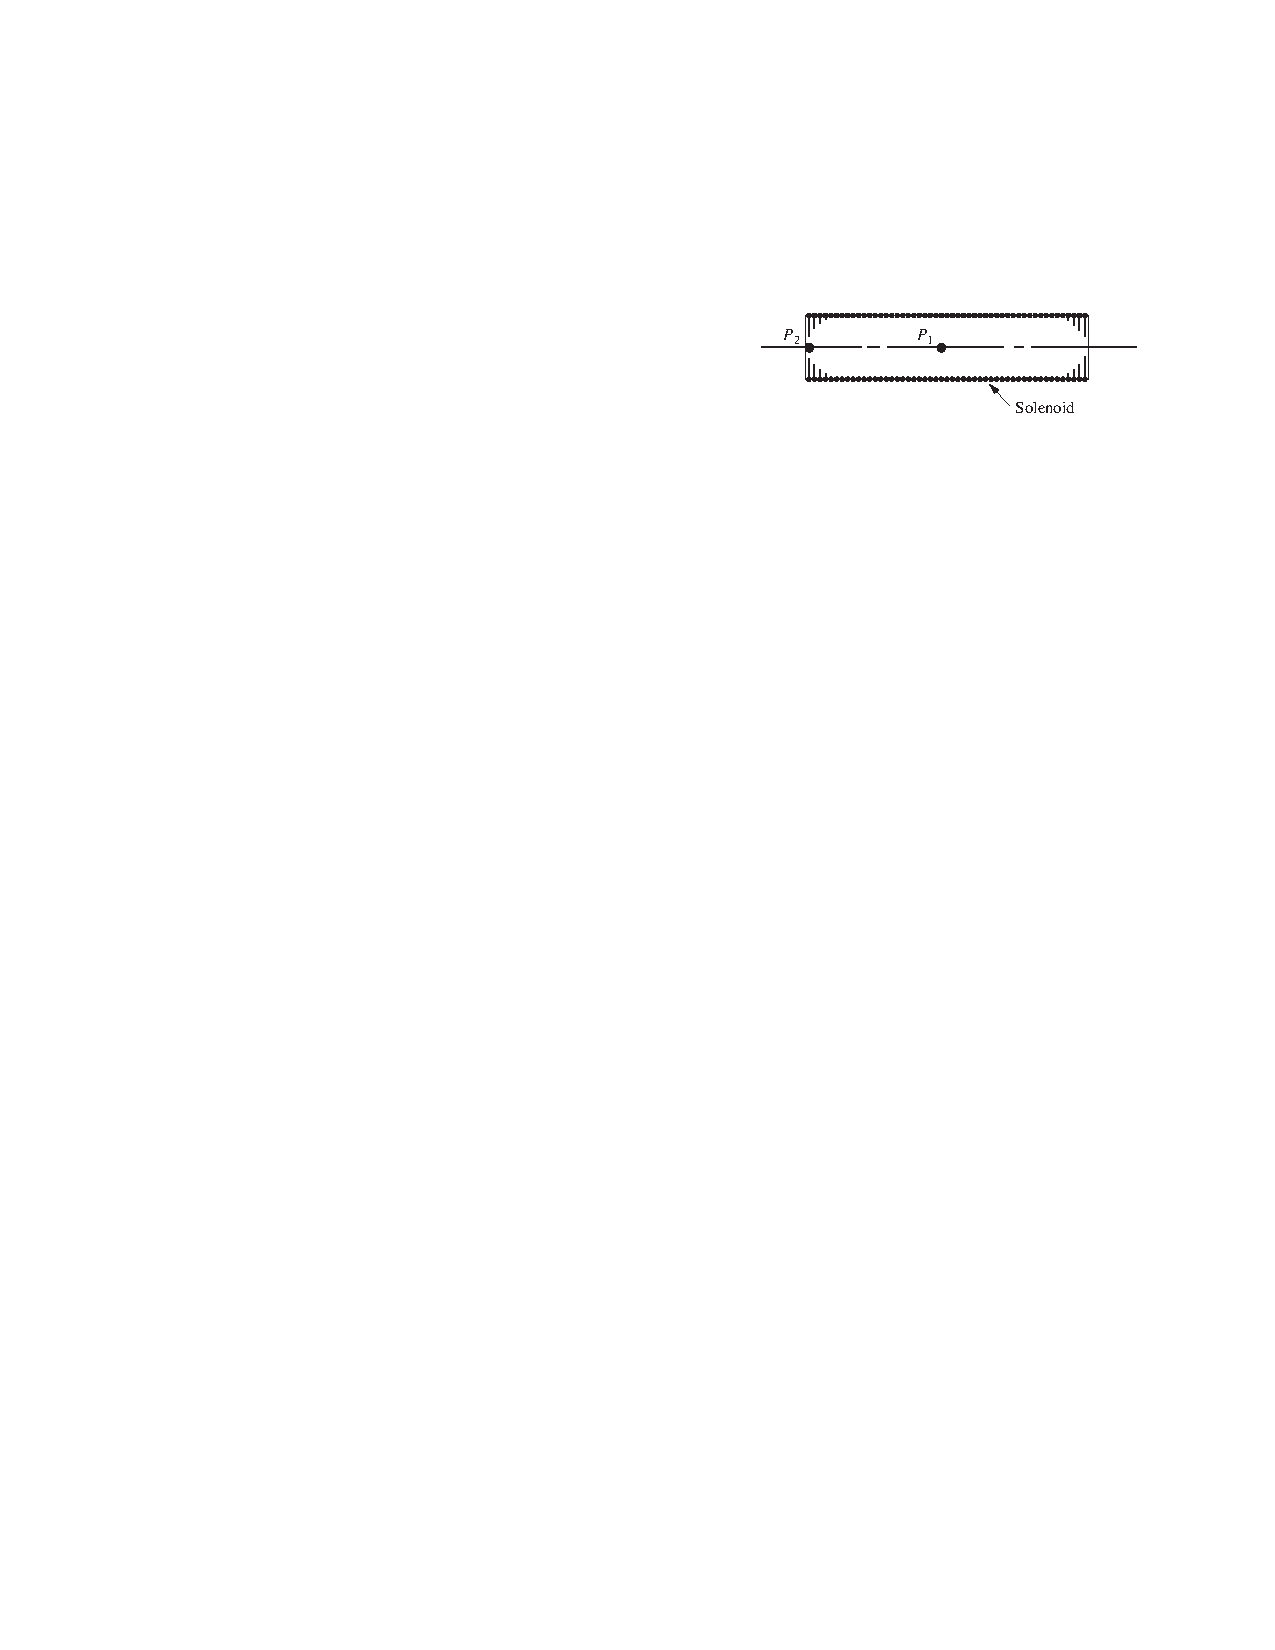
\includegraphics[width=\textwidth]{6_50a.pdf}
			\caption*{Figure~6.50(a)}
		\end{subfigure}
		\begin{subfigure}[b]{0.3\textwidth}
			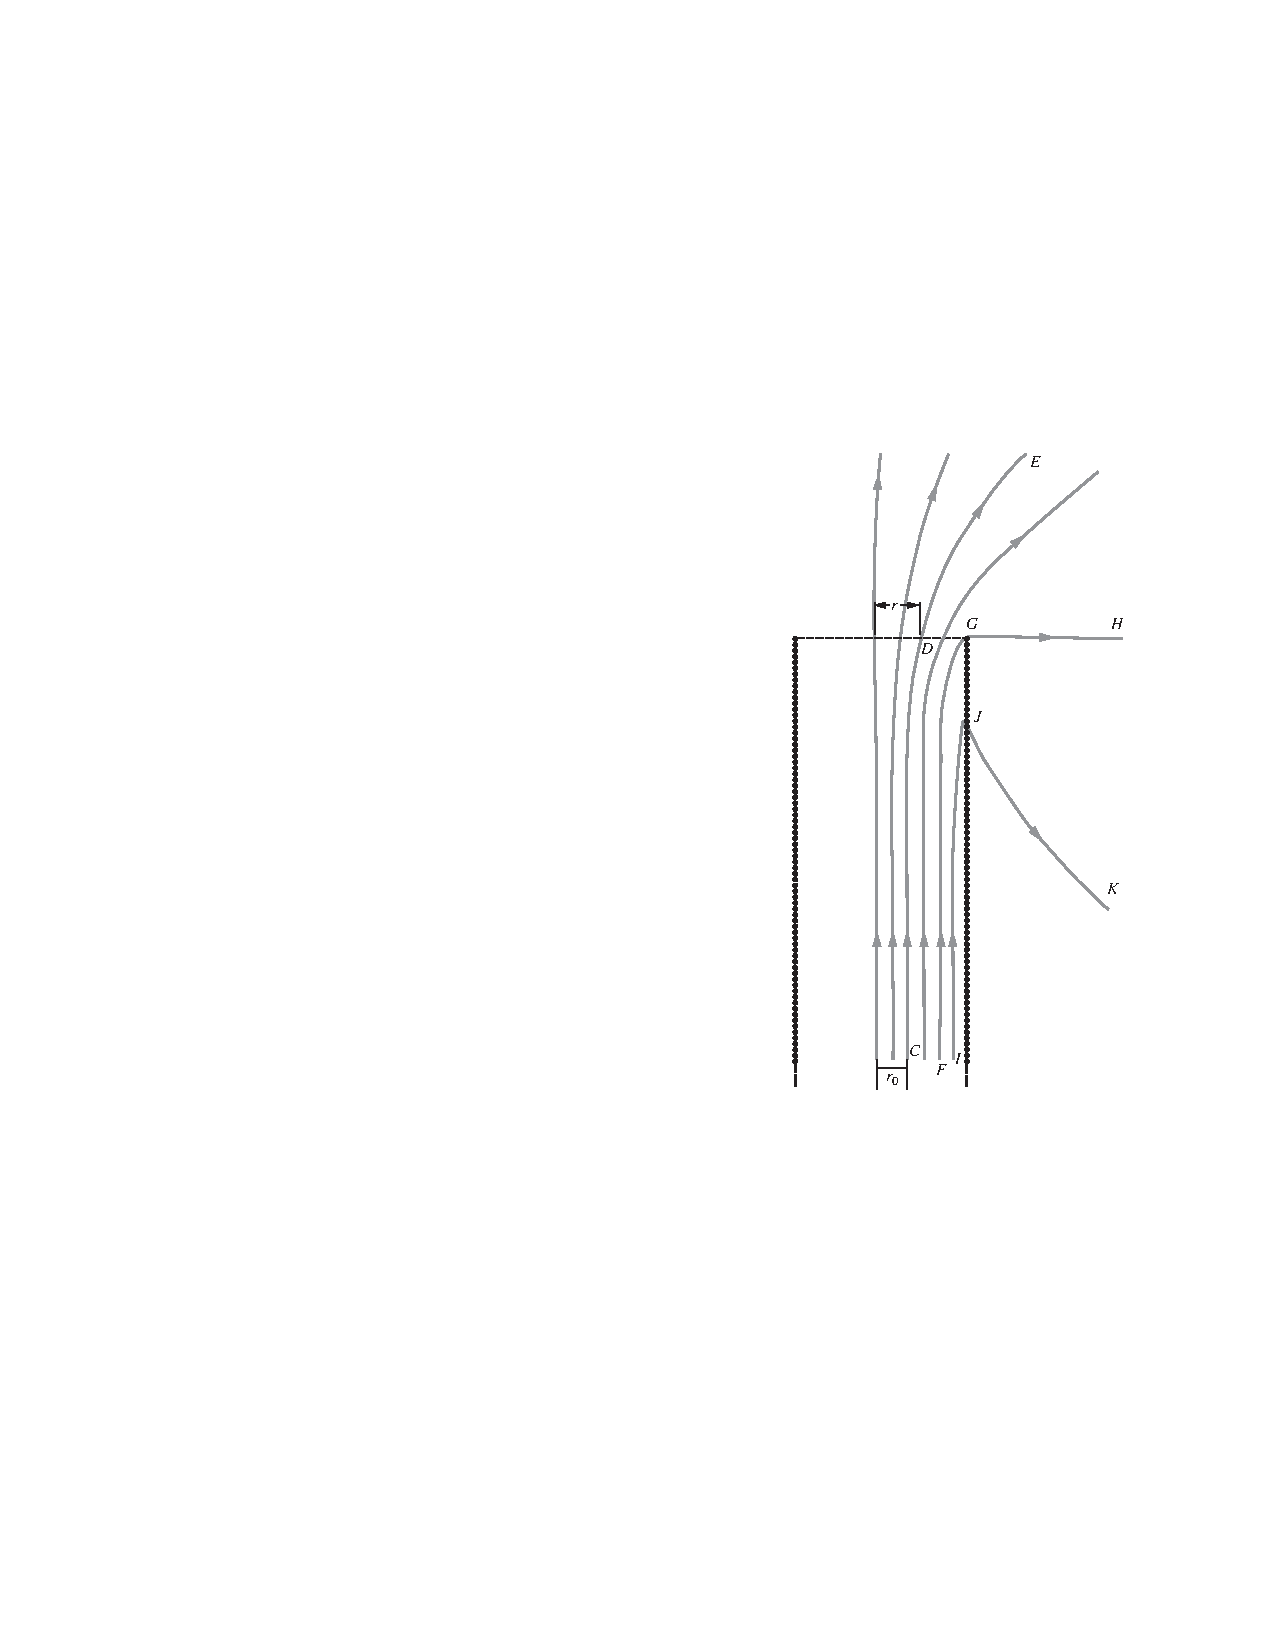
\includegraphics[width=\textwidth]{6_50b.pdf}
			\caption*{Figure~6.50(b)}
		\end{subfigure}
	\end{figure}
	% Question

	\textbf{Solution}
	\begin{enumerate}[label=(\alph*)]
		\item Imagine two solenoids connected to each other at $P_2$. As uniform as this, the field at $P_2$ should equal to that at $P_1$. Now take one of the two solenoids away, and then $P_2$ should be approximately half the field at $P_1$ now. Because of the leakage of field lines, it should be slightly less than half.
		\item If another semi-infinite solenoid is put above this one, then the field should add up to zero. Because of this plane symmetry of the configuration at the junction, the field of each solenoid must be lying in the junction plane, in opposite direction and have the same magnitude. The only way of this is the configuration shown in the figure.
		\item Similarly, if another semi-infinite solenoid is put above this one, then the flux at this plane should now equal to the plane back in the interior, as they are a whole now. Take the upper solenoid away, and half the flux is left.
		\item Consider a loop of radius $r_0$ inside an infinite solenoid. In this near uniform field the flux enclosed should be $B\pi{r_0}^2$. Now cut the solenoid half, and the field at the section becomes $B/2$. To maintain the same flux, $\frac{B}{2}\pi\left(\sqrt{2}r_0\right)^2$. The distance from the axis of the same field line out of the solenoid is now $\sqrt{2}r_0$.
	\end{enumerate}
\end{homeworkProblem}

%----------------------------------------------------------------------------------------
%	PROBLEM 6
%----------------------------------------------------------------------------------------

\begin{homeworkProblem}
	(6.70) \textit{Drifting motion}

	Figure~6.52 shows the path of a positive ion moving in the $xy$ plane. There is a uniform magnetic field of 6000 gauss in the $z$ direction. Each period of the ion's cycloidal motion is completed in 1 microsecond. What are the magnitude and the direction of the electric field that must be present? \textit{Hint:} Think about a frame in which the electric field is zero.
	\begin{figure}[H]
		\centering
		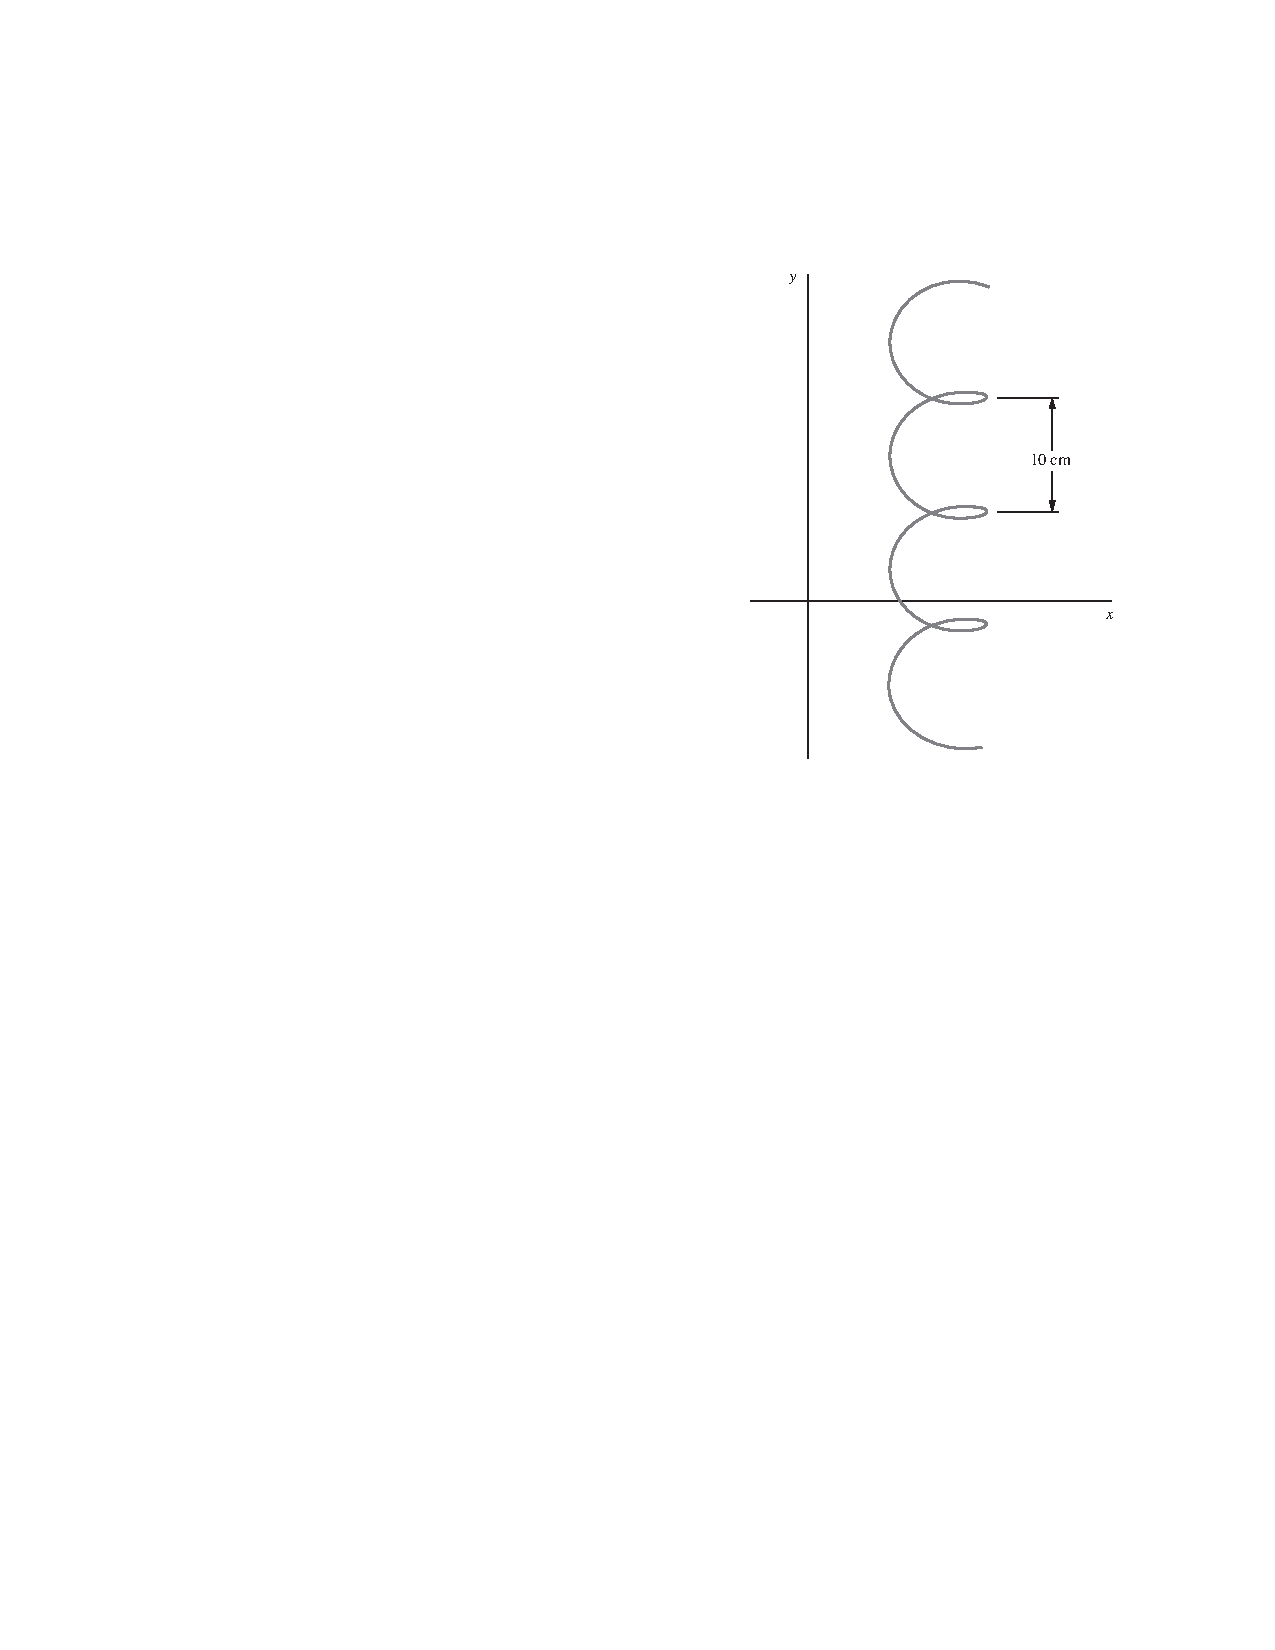
\includegraphics[width = 0.3\textwidth]{6_52.pdf}
		\caption*{Figure~6.52}
	\end{figure}
	% Question

	\textbf{Solution}

	Think about a frame $F'$ in which the electric field is zero. That is ${E_x}'=0$. In this frame the ion would be moving in circular motion without drift. So the relative velocity between the two frames is
	\[
		v_r=\frac{s}{T}=\frac{\SI{0.1}{\m}}{\SI{1e-6}{\s}}=\SI{1e5}{\m\per\s}
	\]
	The transformation between the two frames, as shown in equation (6.72), is
	\[
		{E_x}'=\gamma(E_x-v_rB_z)
	\]
	So
	\[
		E_x=v_rB_z=\SI{1e5}{\m\per\s}\times\SI{0.6}{\tesla}=\SI{6e4}{\newton\per\coulomb}
	\]
\end{homeworkProblem}

%----------------------------------------------------------------------------------------

\end{document}
